\documentclass[aspectratio=169]{beamer}

%%%%%
%%%%%
%%%%%     DEFINE THE THEME USED
%%%%%
%%%%%

\usetheme{jc}

%%%%%
%%%%%
%%%%%     LIST OF PACKAGES USED
%%%%%
%%%%%

\graphicspath{{imgs/}}

\usepackage[utf8]{inputenc}
\usepackage[T1]{fontenc}

\usepackage[]{nicefrac}

\usepackage[]{amsmath, amssymb, amsfonts}
\usepackage[]{bm}

\usepackage[]{graphicx}

\usepackage{tikz}
\usetikzlibrary{shapes}

\DeclareMathOperator*{\minimize}{minimize~}
\DeclareMathOperator*{\maximize}{maximize~}
\DeclareMathOperator*{\subto}{subject~to~}

%%%%%
%%%%%
%%%%%     INFO ABOUT THE PRESENTATION
%%%%%
%%%%%

\title{On the importance of low-dimensional structures for data-driven modeling}
\author[JC]{Jean-Christophe Loiseau}
\date[]{May, 13\textsuperscript{th} 2022}

%%%%%
%%%%%
%%%%%     PRESENTATION
%%%%%
%%%%%

\begin{document}

\begin{frame}
  \titlepage
\end{frame}

%% \begin{frame}[t, c]{blabla}
%%   \vfill

%%   \centering
  
%%   This is a test

%%   \vfill
  
%%   \begin{tcolorbox}[enhanced, coltitle=black, coltext=white, colback=black, title=My title, frame style tile={width=\paperwidth}{background.jpg}]
%%     Hello
%% \end{tcolorbox}
  
%%   \vfill
%% \end{frame}

\begin{frame}{Who am I ?}
  \vfill
  \begin{minipage}{.68\textwidth}
    \begin{itemize}
    \item Maître de Conférences in Fluid Dynamics and Applied Math.

      \bigskip

    \item Machine-learning enthusiast with application to engineering systems.

      \bigskip

    \item Data-efficient models with guarantees of optimality or interpretability.
    \end{itemize}
  \end{minipage}%
  \hfill
  \begin{minipage}{.28\textwidth}
    \includegraphics[width=\textwidth]{myself}
  \end{minipage}
  
  \vfill
\end{frame}

{
  \setbeamercolor*{background canvas}{bg=white}

\begin{frame}%{A gallery of fluid motion}
  \vfill
  \begin{minipage}{.68\textwidth}
    \centering
    \includegraphics[width=\textwidth]{snapshot_re125_0}
    
    {\small \textcolor{black}{Aerodynamics}}

    \bigskip
    
    \includegraphics[width=\textwidth]{tic_m=1_fourier_mode_snapshot}

    {\small \textcolor{black}{Rocket science}}
  \end{minipage}%
  \hfill
  \begin{minipage}{.28\textwidth}
    \centering
    \includegraphics[width=\textwidth]{temperature_field_00000}

    {\small \textcolor{black}{Heat exchange}}
  \end{minipage}
  
  \vfill
\end{frame}
}

\begin{frame}{N.\ Wiener's classification}
  \centering
  \vfill

  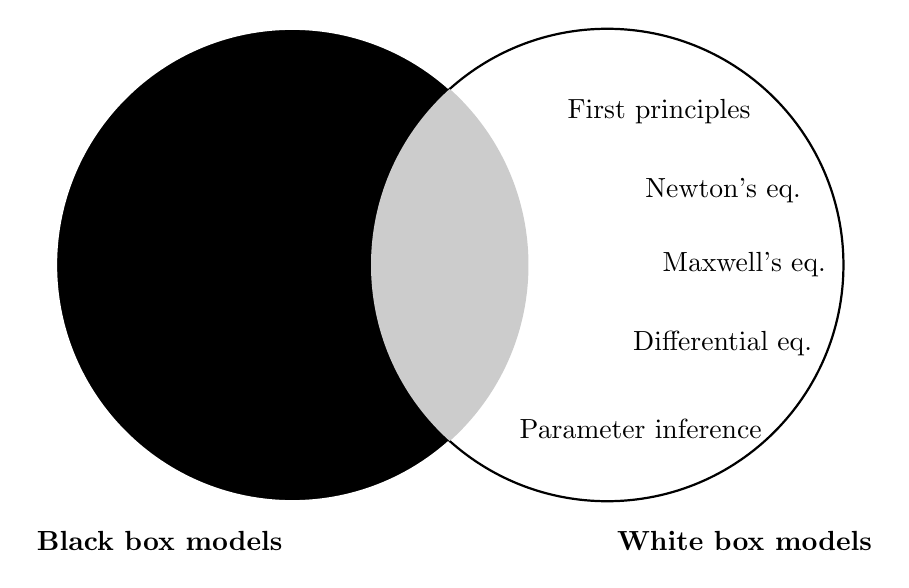
\begin{tikzpicture}
    %\draw[help lines, step=1] (-7, -3) grid (7, 3);

    \draw[thick, white, fill=black] (-2, 0) circle (3);
    \draw[thick, black,fill=white] (2, 0) circle (3);

    \begin{scope}
      \clip (-2, 0) circle (3);
      \clip (2, 0) circle (3);
      \fill[thick, black, fill=gray!40] (0, 0) circle (3);
    \end{scope}

    \node[anchor=east] at (-2, -3.5) {\textbf{Black box models}};
    \node[anchor=west] at (2, -3.5) {\textbf{White box models}};

    \node at (-2, 0) (A) {};
    \path (A) ++(135:2.75) node[anchor=west] {Feedforward nets};
    \path (A) ++(160:2.95) node[anchor=west] {Reinforcement};
    \path (A) ++(170:2.8) node[anchor=west] {learning};
    \path (A) ++(195:2.95) node[anchor=west] {Image classification};
    \path (A) ++(220:2.95) node[anchor=west] {Model-free inference};


    \node at (2, 0) (B) {};
    \path (B) ++(45:2.75) node[anchor=east] {\textcolor{black}{First principles}};
    \path (B) ++(20:2.75) node[anchor=east] {\textcolor{black}{Newton's eq.}};
    \path (B) ++(0:2.9) node[anchor=east] {\textcolor{black}{Maxwell's eq.}};
    \path (B) ++(-20:2.9) node[anchor=east] {\textcolor{black}{Differential eq.}};
    \path (B) ++(-45:2.95) node[anchor=east] {\textcolor{black}{Parameter inference}};

  \end{tikzpicture}
  
  \vfill
\end{frame}

\begin{frame}{Example: Face recognition}
  two faces with arrows
\end{frame}

\begin{frame}{Example: Face recognition}
  overview figure of the SIAM paper
\end{frame}

\begin{frame}{Example: System identification}
  
\end{frame}

\section{A brief overview of SVD}
\begin{frame}
  \sectionpage
\end{frame}

\begin{frame}
  \vfill

  
  \begin{tcolorbox}[
    enhanced,
    coltitle=black,
    coltext=white,
    colback=black,
    title=\textbf{Singular value decomposition},
    frame style tile={width=\paperwidth}{background.jpg}
    ]

    \begin{overprint}

      \onslide<1>
      \large
      \[
      \bm{A} = \bm{U} \boldsymbol{\Sigma} \bm{V}^T
      \]

      \onslide<2>
      \large
      \[
      \begin{bmatrix}
        \bm{0} & \bm{A} \\
        \bm{A}^T & \bm{0}
      \end{bmatrix}
      \begin{bmatrix}
        \bm{u}_i \\ \bm{v}_i
      \end{bmatrix}
      =
      \sigma_i
      \begin{bmatrix}
        \bm{u}_i \\ \bm{v}_i
      \end{bmatrix}
      \]

    \end{overprint}
  \end{tcolorbox}

  \bigskip
  
  Generalization of the \emph{eigenvalue decomposition} to \textbf{non-square matrices} by E. Beltrami (1873) and C. Jordan (1874).
  The first efficient numerical algorithm was developed by G.\ Golub \emph{et al.} in the late 1960s.
  
  \vfill
\end{frame}

\begin{frame}
  Schematic SVD
\end{frame}

\begin{frame}{Geometric interpretation}

\end{frame}

\begin{frame}{Ordinary least-squares}
  \vfill
  \begin{minipage}{.48\textwidth}
    \begin{overprint}
      \onslide<1>
      \Large
      \[
      \minimize_{\bm{x}} \dfrac{1}{2} \| \bm{Ax} - \bm{b} \|_2^2
      \]

      \onslide<2>
      \Large
      \[
      \hat{\bm{x}} = \bm{A}^{\dagger} \bm{b}
      \]

      \onslide<3>
      \Large
      \[
      \hat{\bm{x}} = \bm{V} \boldsymbol{\Sigma}^{-1} \bm{U}^T \bm{b}
      \]
    \end{overprint}
  \end{minipage}%
  \hfill
  \begin{minipage}{.48\textwidth}
    \large
    \[
    \begin{bmatrix}
      ~ & ~ & ~ & ~ & ~ \\
      ~ & ~ & ~ & ~ & ~ \\
      ~ & ~ & ~ & ~ & ~ \\
      ~ & ~ & ~ & ~ & ~ \\
      ~ & ~ & \bm{A} & ~ & ~ \\
      ~ & ~ & ~ & ~ & ~ \\
      ~ & ~ & ~ & ~ & ~ \\
      ~ & ~ & ~ & ~ & ~ \\
      ~ & ~ & ~ & ~ & ~
    \end{bmatrix}
    \begin{bmatrix}
      ~ \\ ~ \\ \bm{x} \\ ~ \\ ~
    \end{bmatrix}
    =
    \begin{bmatrix}
      ~ \\ ~ \\ ~ \\ ~ \\ \bm{b} \\ ~ \\ ~ \\ ~ \\ ~
    \end{bmatrix}
    \]
  \end{minipage}
  \vfill
\end{frame}

\begin{frame}{Low-rank approximation}
  \vfill

  \begin{minipage}{.48\textwidth}
    \begin{overprint}
      \onslide<1>
      \Large
      \[
      \begin{aligned}
        \minimize_{\hat{\bm{A}}} & \| \bm{A} - \hat{\bm{A}} \|_F^2 \\
        \subto & \mathrm{rank~} \hat{\bm{A}} = r
      \end{aligned}
      \]
      
      \onslide<2>
      \Large
      \[
      \hat{\bm{A}} = \sum_{i=1}^k \sigma_i \bm{u}_i \bm{v}_i^T
      \]
    \end{overprint}
  \end{minipage}%
  \hfill
  \begin{minipage}{.48\textwidth}
  \end{minipage}

  \vfill
\end{frame}

\begin{frame}{Orthogonal Procrustes problem}
  \vfill
  \begin{minipage}{.48\textwidth}
    \begin{overprint}
      \onslide<1>
      \large
      \[
      \begin{aligned}
        \minimize_{\bm{R}} & \| \bm{RA} - \bm{B} \|_F \\
        \subto & \bm{R}^T \bm{R} = \bm{I}
      \end{aligned}
      \]

      \onslide<2>
      \large
      \[
      \bm{BA}^T = \bm{U} \boldsymbol{\Sigma} \bm{V}^T
      \]

      \onslide<3>
      \large
      \[
      \bm{R} = \bm{UV}^T
      \]

    \end{overprint}
  \end{minipage}%
  \hfill
  \begin{minipage}{.48\textwidth}
    \includegraphics[width=\textwidth]{procrustes}
  \end{minipage}
  \vfill
\end{frame}

\section{SVD in data-driven modeling}
\begin{frame}
  \sectionpage
\end{frame}

\begin{frame}
  \vfill

  \Large

  \[
  \bm{y} = \bm{Kx} + \varepsilon
  \]

  \vfill
\end{frame}

\begin{frame}{Linear deconvolution problem}
  Schematic of a linear system
\end{frame}

\begin{frame}{Linear deconvolution problem}
  Schematic of deconvolution
\end{frame}

\begin{frame}
  \vfill

  \Large

  \[
  \bm{y} = \bm{Kx} + \varepsilon
  \]

  \vfill
\end{frame}

\begin{frame}

\end{frame}

\begin{frame}

  \vfill

  \begin{tcolorbox}[
      enhanced,
      coltitle=black,
      coltext=white,
      colback=black,
      title=\textbf{Fundamental problem of component analysis},
      frame style tile={width=\paperwidth}{background.jpg}
    ]

    \begin{overprint}
      \onslide<1>
      \large
      \[
      \begin{aligned}
        \minimize_{\bm{K}} & \| \bm{M}^{\frac12} \left( \bm{Y} - \bm{KX} \right) \|_F \\
        \subto & \mathrm{rank~} \bm{K} = r.
      \end{aligned}
      \]

      \onslide<2>
      \large
      \[
      \begin{aligned}
        \minimize_{\bm{P}, \bm{Q}} & \| \bm{M}^{\frac12}  \left( \bm{Y} - \bm{PQ}^T \bm{X} \right) \|_F \\
        \subto & \bm{P}^T \bm{MP} = \bm{I}_r \quad \left( \mathrm{ou~} \bm{Q}^T \bm{XX}^T \bm{Q} = \bm{I}_r \right).
      \end{aligned}
      \]

    \end{overprint}

  \end{tcolorbox}

  \vfill
\end{frame}

\begin{frame}
  \vfill

  \Large
  \[
  \begin{bmatrix}
    \bm{M} & \bm{0} \\
    \bm{0} & \bm{0}
  \end{bmatrix}
  \begin{bmatrix}
    \bm{p}_i \\ \bm{q}_i
  \end{bmatrix}
  \lambda_i
  =
  \begin{bmatrix}
    \bm{0} & \bm{M} \bm{C}_{\bm{yx}} \\
    \bm{C}_{\bm{xy}} \bm{M} & - \bm{C}_{\bm{xx}}
  \end{bmatrix}
  \begin{bmatrix}
    \bm{p}_i \\ \bm{q}_i
  \end{bmatrix}
  \]

  \vfill
\end{frame}

\begin{frame}{Proper Orthogonal Decomposition}
  \vfill

  \begin{minipage}{.38\textwidth}
    \begin{tcolorbox}[
        enhanced,
        coltitle=black,
        coltext=white,
        colback=black,
        title=\textbf{POD eigenproblem},
        frame style tile={width=\paperwidth}{background.jpg}
      ]
      \large
      \[
      \bm{M} \bm{p}_i \lambda_i = \bm{C}_{\bm{xx}} \bm{p}_i
      \]

      \smallskip
    \end{tcolorbox}
  \end{minipage}%
  \hfill
  \begin{minipage}{.58\textwidth}
    POD is recovered if $\bm{X} = \bm{Y}$ and $\bm{P} = \bm{Q}$.
    It aims at characterizing the second order statistics of the random variable $\bm{x}$.
  \end{minipage}

  \vfill
\end{frame}

\begin{frame}
  \vfill

  \begin{minipage}{.48\textwidth}

    \centering
    \textbf{Complex Ginzburg-Landau equation}

    \[
    \dfrac{\partial q}{\partial t} = -U \dfrac{\partial q}{\partial x} + \mu(x) q + \gamma \dfrac{\partial^2 q}{\partial x^2} - \beta \vert q \vert^2 q
    \]
  \end{minipage}%
  \hfill
  \begin{minipage}{.48\textwidth}
  \end{minipage}

  \vfill
\end{frame}

\begin{frame}
  \vfill

  \begin{minipage}{.48\textwidth}
    Covariance matrix
  \end{minipage}%
  \hfill
  \begin{minipage}{.48\textwidth}
    Eigenspectrum
  \end{minipage}

  \vfill
\end{frame}

\begin{frame}
  \vfill

  \begin{minipage}{.48\textwidth}
    POD mode
  \end{minipage}%
  \hfill
  \begin{minipage}{.48\textwidth}
    Phase portrait
  \end{minipage}

  \vfill
\end{frame}

\end{document}
